\section{Анализ предметной области}

%Прежде чем приступить к обзору и анализу существующих средств сетевого мониторинга ядра Linux, необходимо определить что подразумевается под сетевым мониторингом ядра Linux.

\subsection{Ядро Linux}
Ядро Linux --- основной внутренний компонент ОС Linux, отвечающие за поддержку работу с накопителями, управление работы процессора посредством переключения между выполняемыми задачами, распределение системными ресурсами, управление аппаратным обеспечением и обеспечение взаимодействие приложения с аппаратным обеспечением, а также ядро принимает сообщения и пакеты данных из сети и отправляет их в сеть~\cite{kernel_linux_robert}.

Прежде всего для ядра ставятся задачи обеспечение среды выполнения для программ в ОС, взаимодействие с аппаратными компонентами и обслуживание их низкоуровневые элементы.
Кроме того в настоящее время в функции ядра включают управление процессорами графической оболочки, обеспечивающей интерфейс между пользователем и ОС.

Ядро Linux является монолитным с модульной конструкцией, которое реализовано в виде одного процесса, выполняющий в одном адресном пространстве.
Такое ядро обычно хранится на диске в виде одного статического бинарного файла.
Все службы ядра находятся и выполняются в одном большом адресном пространстве ядра.
Взаимодействия в ядре осуществляются очень просто, потому что все, что выполняется в режиме ядра, выполняется в одном адресном пространстве.
В отличие от микроядра, который разделяет службы ядра на несколько процессов, называемыми серверами.
Ядро может вызывать функции непосредственно, как это делают пользовательские приложения.

\subsection{Подсистемы ядра}
Ядро Linux разделяется на ряд подсистем, показанные на рисунке \ref{img:arch_linux}, как на высоком, так и на низких уровнях. Такое разделение позволяет упростить разработку ядра и сделать его более гибким.
Каждая подсистема реализует свой функционал, такие как: управление памятью, управление и взаимодействие процессов, файловая система, сетевые стек, которое используется другими подсистемами. Компоненты системы разнесены по слоям, несмотря на то, что модели или подсистемы работают в <<одном слое>>.

\begin{figure}[h!]
	\centering
	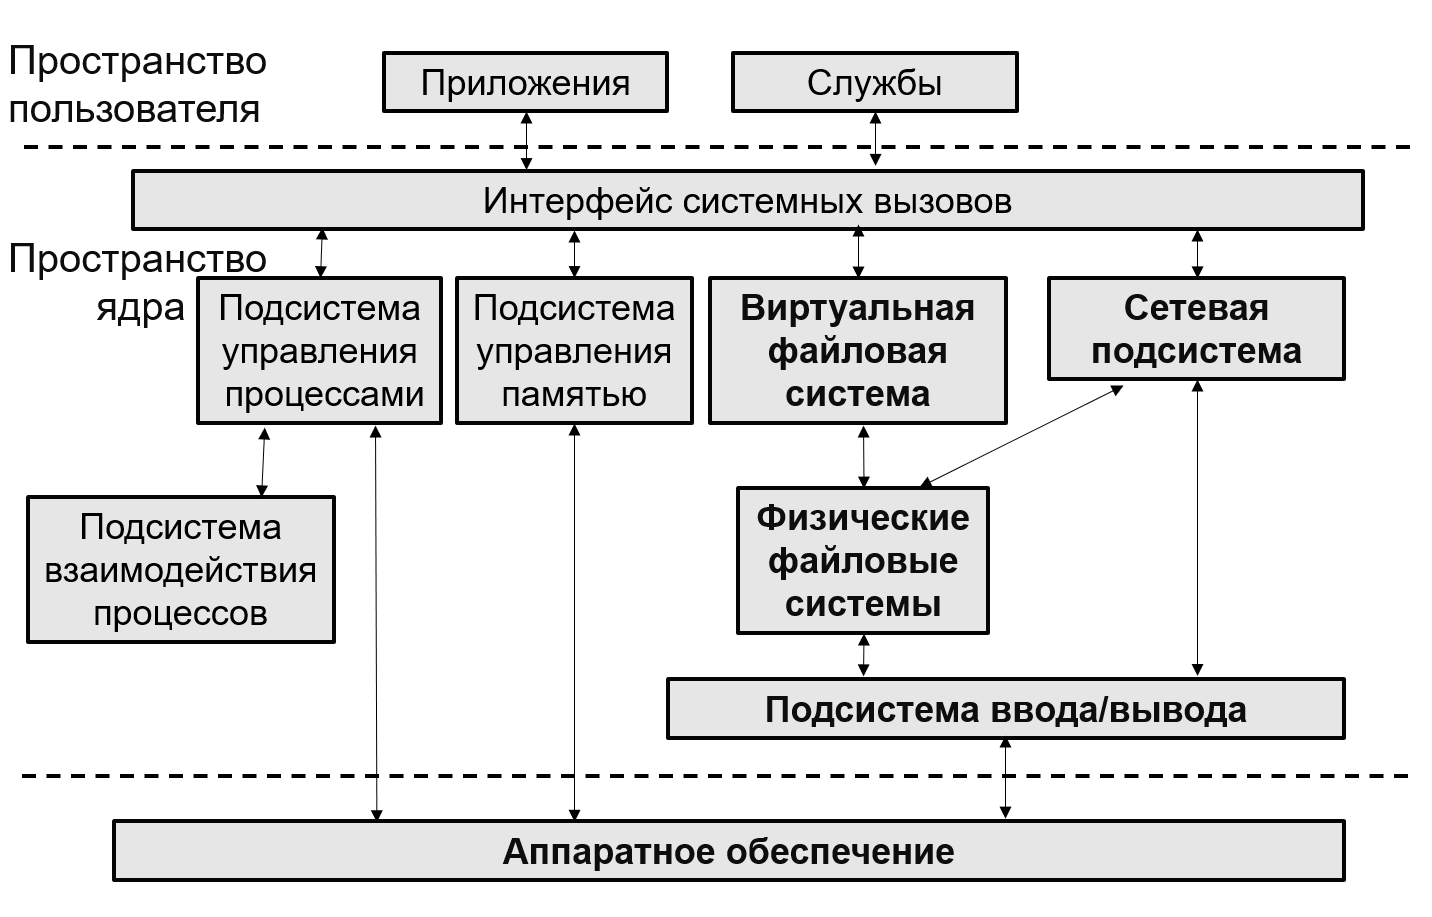
\includegraphics[height=0.4\textheight]{img/arch_linux} % height
	\caption{Общая архитектура Linux}
	\label{img:arch_linux}
\end{figure}

В ОС Linux три главных уровня, показанные на рисунке \ref{img:arch_linux}.
В основе расположены аппаратные средства, включающие память, процессор и выполняющие вычисления, запросы на чтение из памяти и запись в нее, а также устройства такие как жесткий диск и сетевые интерфейсы.
Уровнем выше расположено пространство ядро (от англ. kernel space), включающее системные переменные и область памяти ядра. Выше же пользовательские процессы, которыми управляет ядро, называемым пространством пользователя (от англ. user space).

В Linux выделяют два режима работы ее программных средств --- режим ядра (от англ. kernel mode) или привилегированным режимом, и пользовательский режим (от англ. user mode).
Основное различие двух режимов состоит в привилегиях доступа к аппаратным средствам --- оперативной памяти, процессору и устройства ввода-вывода, к которым разрешен полный доступ из режима ядра и ограниченный доступ из пользовательского режима. Это сильное преимущество, но может быть опасным, поскольку позволяет процессам ядра с легкостью нарушить работу всей системы.
В режиме пользователя, для сравнения, доступен ограниченный объем памяти и разрешены безопасные инструкции для процессора.
Пространством пользователя называют участки оперативной памяти, которые могут быть доступны пользовательским процессам. Если какой-либо процесс завершается с ошибкой, ее последствия будут ограниченными и ядро сможет их очистить. Это означает, что, если, например, произойдет сбой в работе браузера, выполнение научных расчетов, которые вы запустили на несколько дней в фоновом режиме, не будет нарушено.

\subsection{Сетевая подсистема ядра}

Сетевая подсистема ядра Linux \cite{moduls_kernel_linux, linux_network_internals} обеспечивает взаимодействие процессов, выполняющихся на разных узлах сети, то есть дает возможность сетевого взаимодействия между приложениями.

Сетевая подсистема ядра Linux реализует следующую функциональность:
\begin{itemize}
	\item поддержку взаимодействия процессов с помощью механизмов сокетов (sockets);
	\item реализацию стеков сетевых протоколов (TCP/IP, UDP/IP, IPX/SPX и другие);
	\item поддержку сетевых интерфейсов или драйверов;
	\item обеспечение маршрутизации пакетов (routing);
	\item обеспечение фильтрации пакетов (netfilter).
\end{itemize}

\subsubsection{Состав подсистемы}

В состав сетевой подсистемы входят модули~\cite{os_gostev}, показанные на рисунке~\ref{img:arch_network_subsystem}.

\begin{itemize}
	\item Драйверы сетевых устройств обеспечивают связи с помощью аппаратных средств.
	Для каждого сетевого устройства существует свой драйвер.
	\item Модуль аппаратно-независимого интерфейса обеспечивает пользовательскому процессу единый интерфейс ко всем физическим сетевым устройствам.
	\item Модуль сетевых протоколов предназначен для реализации всех возможных транспортных протоколов в сети.
	\item Модуль интерфейсов независимых от протоколов обеспечивает интерфейсы, которые не зависят от протоколов и физических устройств.
	Этот модуль использует ядро для доступа к сети без привязки к протоколами и физическим устройствам.
	\item Системный интерфейс нужен для взаимодействия ядра или пользователя с сетевой подсистемой.
\end{itemize}

\begin{figure}[h!]
	\centering
	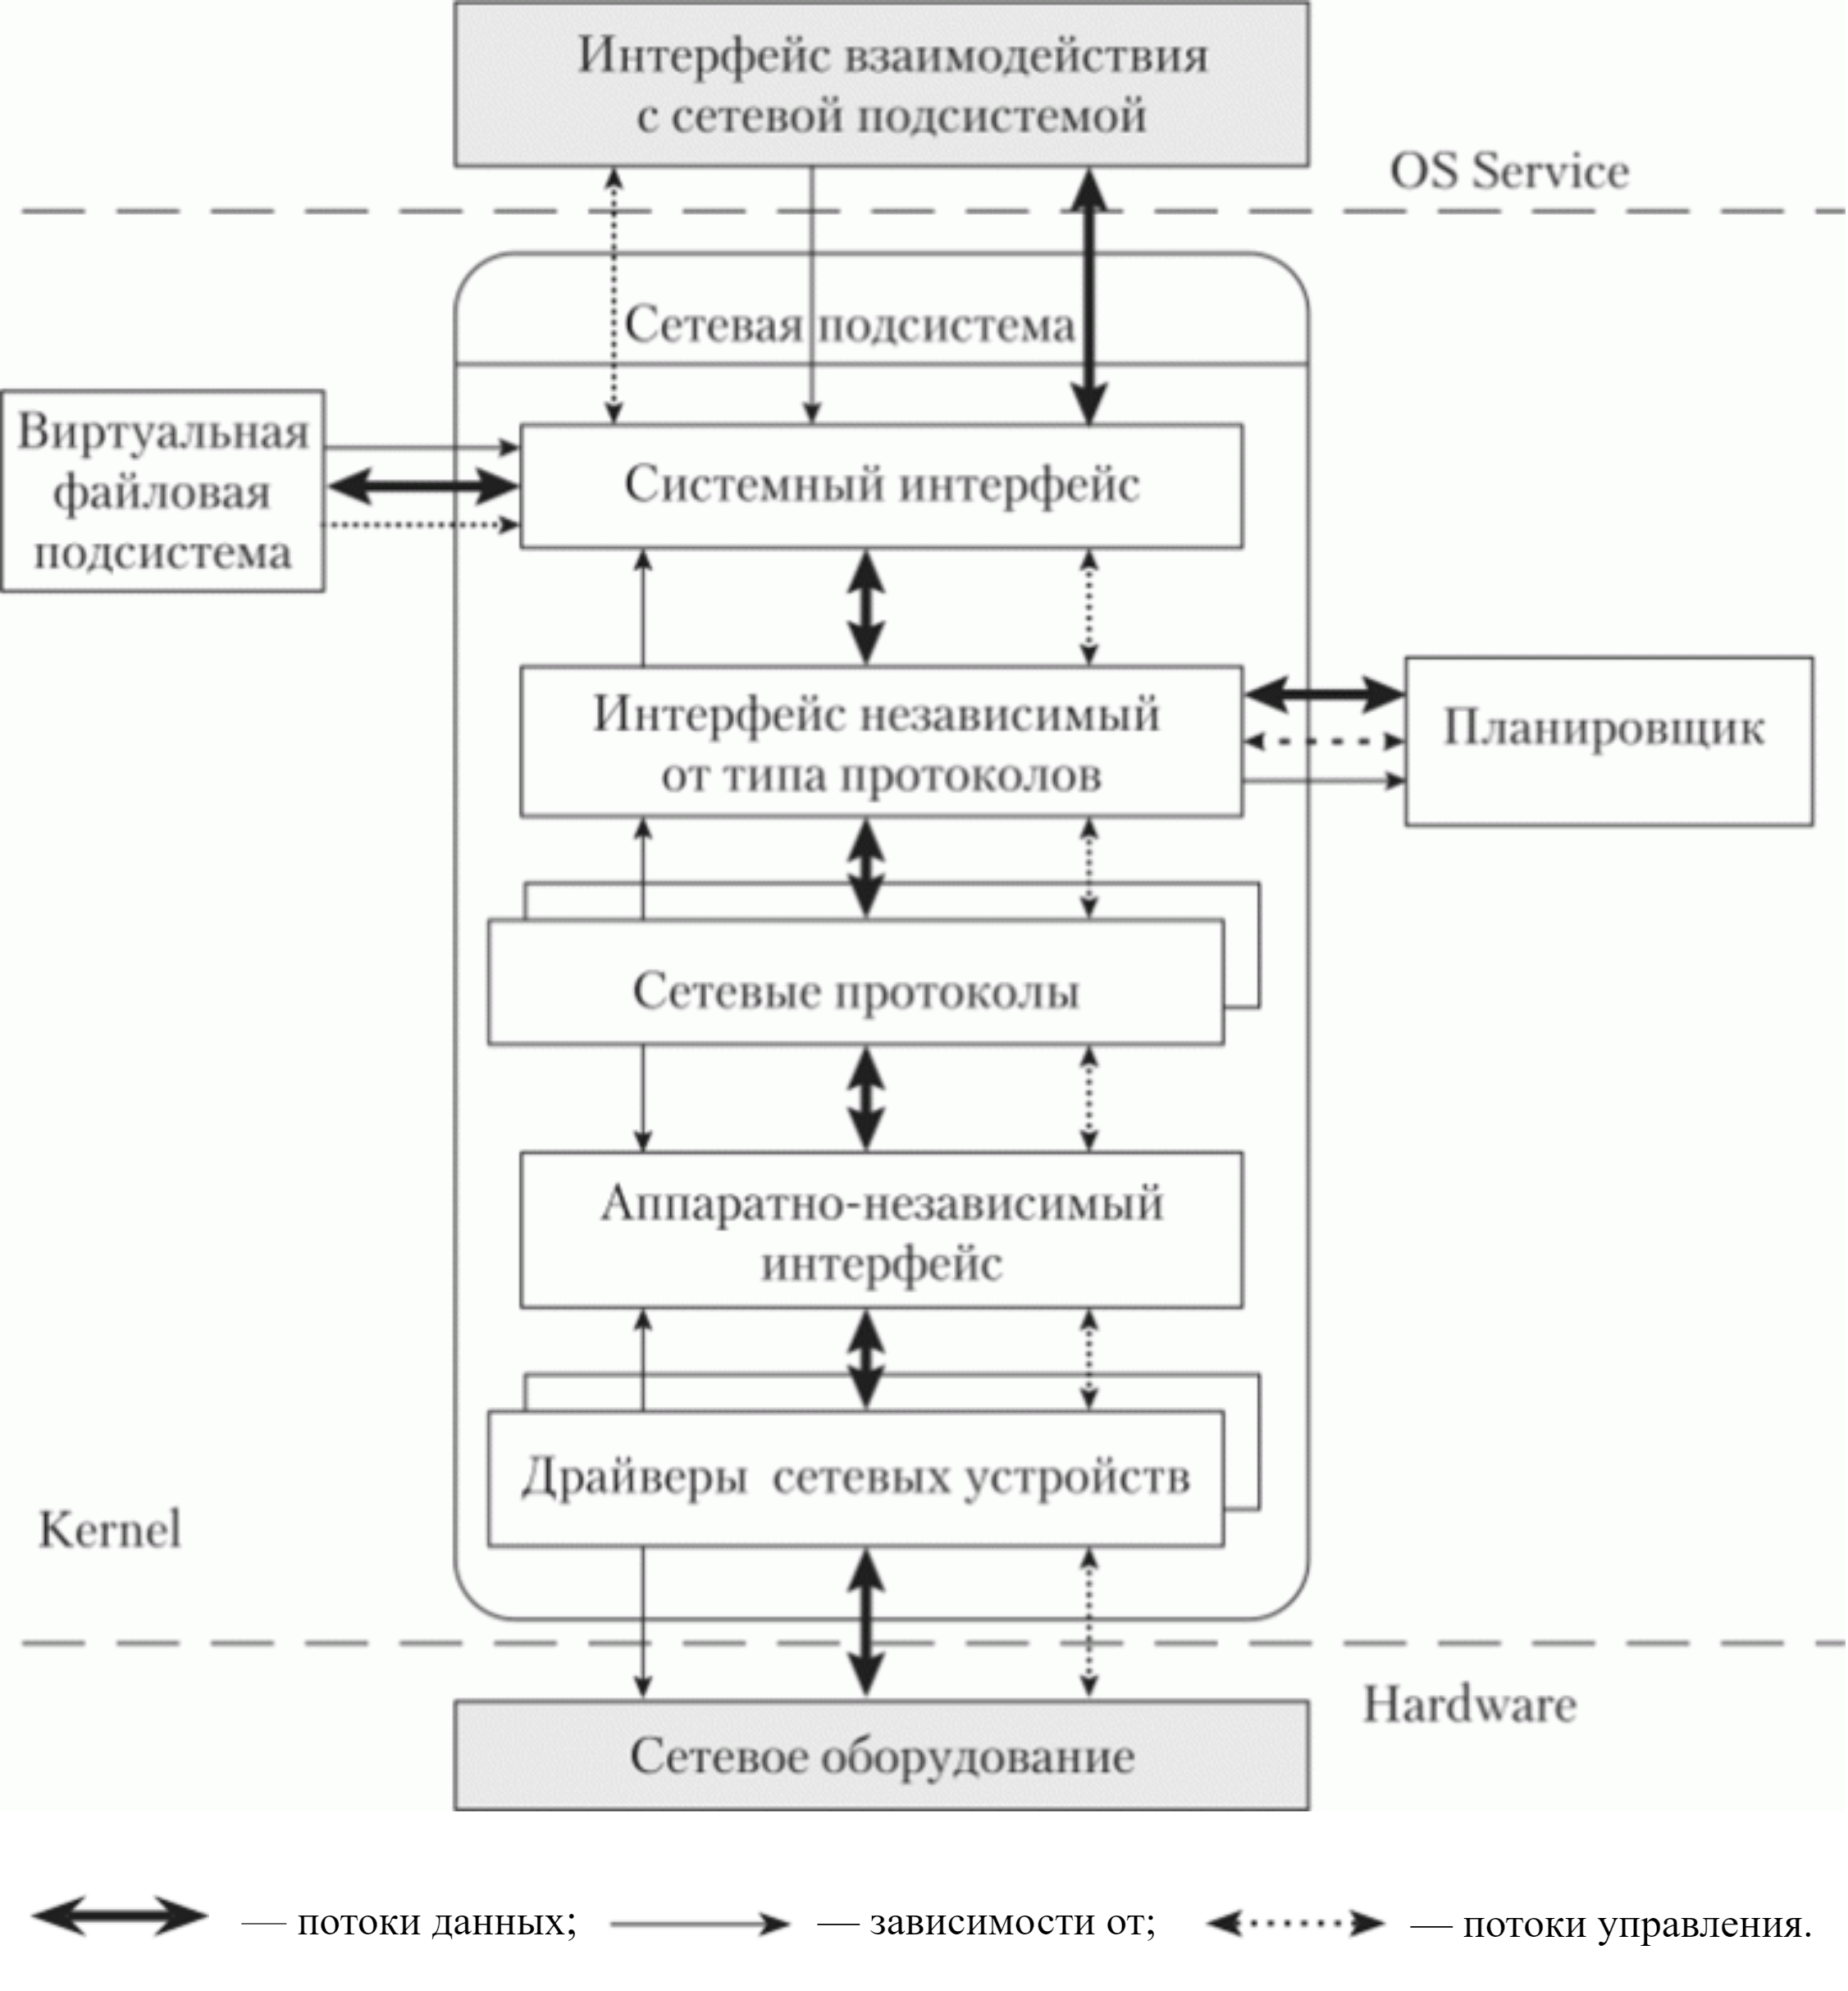
\includegraphics[height=0.45\textheight]{img/arch_network_subsystem} % height
	\caption{Архитектура сетевой подсистемы ядра Linux}
	\label{img:arch_network_subsystem}
\end{figure}

\subsubsection{Зависимости сетевой подсистемы}

Сетевая подсистема обращается к планировщику для приостановления и возобновления работы процессов, пока они находятся в ожидании завершения запроса оборудования, что приводит к зависимости других подсистем.
И применяет планировщик для временной синхронизации функций обмена данными.
Также поддерживает VFS посредством реализации элементов логической файловой системы в части NFS, что приводит к зависимости VFS от сетевой подсистемы и контролю потоков данных между подсистемами.
Сетевая подсистема зависит от IPC, путем использования демона kerneld динамической загрузки и выгрузки исполняемых модулей.

\begin{figure}[h!]
	\centering
	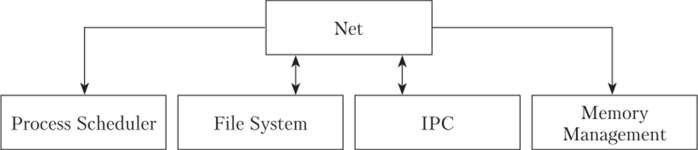
\includegraphics[width=0.8\textwidth]{img/depends_network_subsystem} % width
	\caption{Зависимости сетевой подсистемы}
	\label{img:depends_network_subsystem}
\end{figure}


\subsubsection{Сетевой стек}

Каждый объект в сети, с точки зрения Linux --- сокеты, представляющая собой структуру данных в сетевом узле сети, которая служит конечной точкой для отправки и приема данных по сети. Сетевая подсистема основана на использовании модели сокетов, введенных в OC BSD, и поддерживает множество различных сетевых стеков протоколов.
Данные многоуровневые протоколы применяются для решения задач сетевых взаимодействий, заключающийся в разбиении процесса коммуникации на набор уровней с четко определенными способами взаимодействия уровней на одном узле и на соседних узлах для обеспечения коммуникации различного оборудования.
Реализация сетевой поддержки в ОС-ах основана на структуре сокетов struct socket, содержащая поле идентификатора типа сокета (потоковый или дейтаграммный), состояние сокета (в состоянии соединения или нет), поле с флагами (модифицируют работу сокета), указатель на структуру со списком операций для выполнения сокетом и другие данные. На листинге~\ref{lst:socket_t} показана полная структура сокета.

Сетевая реализация построена так, чтобы не зависеть от конкретики протоколов.
Таким образом в подсистеме существует сетевой стек, который оснащен набором интерфейсов, которые варьируются от протоколо-независимых (protocol agnostic), таких как интерфейс уровня сокетов или уровня устройств, до специальных интерфейсов конкретных сетевых протоколов. 

\begin{lstlisting}[label=lst:socket_t,caption=Структура сокета struct socket \cite{socket_struct}]
struct socket {
	socket_state state;
	short type;
	unsigned long flags;
	struct socket_wq __rcu * wq;
	struct file * file;
	struct sock * sk;
	const struct proto_ops * ops;
};  
\end{lstlisting}	

Уровень сокетов представляет собой стандартный API к различным сетевым протоколам для сетевой подсистемы, обеспечивающий способ управления соединениями и передачи данных между конечными точками, от доступа к данных и блокам данных протокола IP/PDU, и до протоколов TCP/UDP.

В то время как работа в сети отсылается к модели сетевого взаимодействия по OSI, сетевой стек в Linux использует модель TCP/IP \cite{tcpip_craig, tcpip_lora}, включающая в себя 4 уровня:
\begin{enumerate}
	\item уровень сетевых интерфейсов (канальный уровень) относится к драйверам устройств, обеспечивающим доступ к физическому уровню, который может состоять из многочисленных сред, таких как последовательные каналы или устройства Ethernet, описываются как сетевые интерфейсы;
	\item уровень межсетевого взаимодействия (сетевой уровень) обеспечивает работу базовой
	службы доставки пакетов по назначению;
	\item транспортный уровень обеспечивает надежную доставку данных со сквозным обнаружением и устранением ошибок;
	\item прикладной уровень отвечает за взаимодействие с приложениями и процессами на хостах, также определяются пользовательские интерфейсы процесса или приложения, наблюдается работа протоколов и служб --- FTP, Telnet и другие. 
\end{enumerate}

Несмотря на обилие возможностей сетевая подсистема ориентирована на обслуживание протоколов Ethernet и TCP/IP, которые условно вписывается в модель OSI, включающая в себя 7 уровней, показанные на рисунке~\ref{img:protocol}.

\begin{figure}[h!]
	\centering
	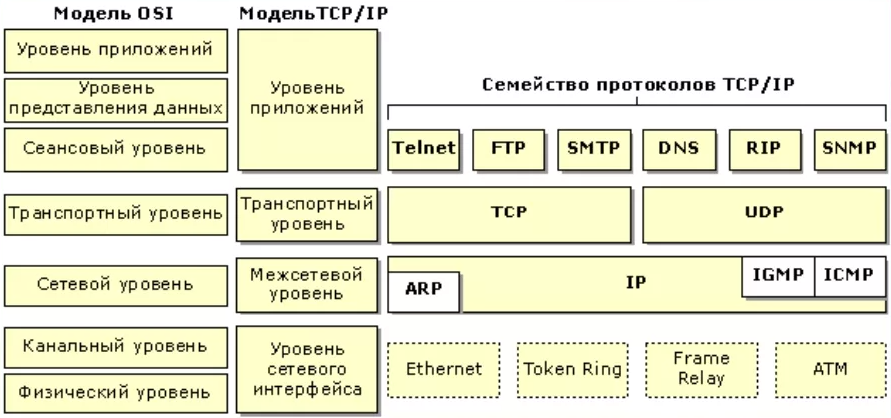
\includegraphics[height=0.3\textheight]{img/protocol}
	\caption{Модель OSI и TCP/IP}
	\label{img:protocol}
\end{figure}

\subsubsection{Сетевые интерфейсы}

Сетевые интерфейсы создаются поддерживающими их драйверами — модулями ядра Linux. В общем случае, разработчик драйвера (модуля ядра) специфического сетевого устройства может выбрать имя для его интерфейса произвольно (определяется драйвером)

Основной структурой данных описывающей сетевой интерфейс --- struct net\_device и представленная на листинге~\ref{lst:net_device}, описанная в <linux/netdevice.h>. Она содержит не только описание аппаратных средств, но и конфигурационные параметры сетевого интерфейса по отношению к протоколам. Данная структура часто меняется от версии к версии ядра.

\clearpage

\begin{lstlisting}[label=lst:net_device,caption=Основная структура данных]
struct net_device { 
	char  name[ IFNAMSIZ ] ; 
	...
	unsigned long  mem_end;   /* shared mem end     */ 
	unsigned long  mem_start; /* shared mem start   */ 
	unsigned long  base_addr; /* device I/O address */ 
	unsigned int   irq;       /* device IRQ number  */ 
	...
	unsigned       mtu;       /* interface MTU value     */ 
	unsigned short type;      /* interface hardware type */ 
	...
	/* Interface address info. */ 
	unsigned char  perm_addr[ MAX_ADDR_LEN ]; /* permanent hw address    */ 
	unsigned char  addr_len;                 /* hardware address length */ 
	...
}
\end{lstlisting}

А вот основной структурой управления передачей пакетов и экземпляров данных между сетевыми уровнями, построена работа всей подсистемы --- буферы сокетов struct sk\_buff, определенная в <linux/skbuff.h> и представленная на листинге~\ref{lst:sk_buff}.
Буфер сокетов состоит их двух частей: данные управления struct sk\_buff и данные пакета, указываемые в struct sk\_buff указателями head и data.~\cite{moduls_kernel_linux, os_gostev}.
В этой структуре объединены все типы пакетов, используемых в сетевой подсистеме, члены которой включают:
\begin{itemize}
	\item счетчики запросов сокета на чтение и запись в память;
	\item флаги, определяющие поведение сокета;
	\item поля управления в буфере;
	\item последовательности действий, предписанным протоколом TCP/IP;
	\item очередь ожидания (struct sk\_queue\_head) для блокирования операций чтения и записи, посредством полей next и prev.
\end{itemize}

\begin{lstlisting}[label=lst:sk_buff,caption=Структура данных управления передачей пакетов]
struct sk_buff {
	struct sk_buff *next;
	struct sk_buff *prev;
	...
	__u16			inner_transport_header;
	__u16			inner_network_header;
	__u16			inner_mac_header;
	__be16			protocol;
	__u16			transport_header;
	__u16			network_header;
	__u16			mac_header;
	...
	sk_buff_data_t		tail;
	sk_buff_data_t		end;
	unsigned char		*head, *data;
	unsigned int		truesize;
	refcount_t			users;
	...
};
\end{lstlisting}

Задача сетевого интерфейса — быть тем местом, в котором:
\begin{itemize}
	\item создаются экземпляры структуры struct sk\_buff, по каждому принятому из интерфейса пакету (здесь нужно принимать во внимание возможность сегментации IP пакетов), далее созданный экземпляр структуры продвигается по стеку протоколов вверх, до получателя пользовательского пространства, где он и уничтожается;
	\item исходящие экземпляры структуры struct sk\_buff, порождённые на верхних уровнях протоколов пользовательского пространства отправляются, а сами экземпляры структуры после этого --- уничтожаться.
	Более детально эти вопросы рассмотрены, при обсуждении прохождения пакетов сквозь стек
	сетевых протоколов.
\end{itemize}

\subsubsection{Путь пакета данных сквозь стек протоколов}

Структура вложенности заголовков сетевых уровней в точности соответствует структуре
инкапсуляции сетевых протоколов протоколов внутри друг друга, это позволяет обрабатывающему
слою получать доступ к информации, относящейся только к нужному ему слою.
Экземпляры данных типа struct sk\_buff во-первых возникают при поступлении очередного сетевого пакета из внешней физической среды распространения данных.
Об этом событии извещает прерывание (IRQ), генерируемое сетевым адаптером. 
При этом создается или извлекается из пула источников экземпляр буфера сокета, заполняется данными из поступившего пакета. Все эти действия выполняются не в самом обработчике верхней половины прерываний от сетевого адаптера, а в обработчике отложенного прерывания NET\_RX\_SOFTIRQ. Затем этот экземпляр дальше вверх от сетевого слоя к слою, до приложения прикладного уровня, которое является получателем пакета. 
На этом экземпляр данных буфера сокета уничтожается.
Во-вторых возникают в среде приложения прикладного уровня, которое является отправителем пакета данных. Пакет помещается в созданный буфер сокета, который начинает перемещаться вниз от сетевого слоя к слою, до достижения канального уровня, где осуществляется физическая передача данных пакета через сетевой адаптер в среду распространения. 
В случае успешного завершения передачи буфер сокета уничтожается. 
При отсутствии подтверждения отправки (IRQ) обычно делается несколько повторных попыток, прежде, чем принять решение об ошибке канала.

\subsection{Сетевой мониторинг ядра}

Сетевой мониторинг ядра Linux --- отслеживание пути пакетов и выявление наличие ошибок сетевых интерфейсов сетевой подсистемы, что относится к вмешательству в работу сетевой подсистемы.
С одной стороны большинство проблем с сетью возникают как раз на физическом и канальном уровнях, но с другой стороны приложения, работающие с сетью оперируют на уровне TCP сессий и не видят, что происходит на более низких уровнях.
Поэтому путем использования сетевого мониторинга можно выявить:
\begin{itemize}
	\item проблемы производительности диска (хранилища);
	\item проблемы производительности памяти и процессора;
	\item узкие места в сети.
\end{itemize}

Сетевой стек устроен сложно, и не существует универсального решения на все случаи жизни.
Если  критически важны производительность и корректность при работе с сетью, то придется потратить немало времени, сил и средств в то, чтобы понять, как взаимодействуют друг с другом различные части системы. 

В идеале следует измерять потери пакетов на каждом уровне сетевого стека. 
В этом случае необходимо выбрать, какие компоненты нуждаются в настройке. Именно на этом моменте, как мне кажется, сдаются многие.
В ряде случаев, вероятно, система бывает настолько пронизана взаимосвязями и наполнена нюансами, что если вы пожелаете реализовать полезный мониторинг или выполнить настройку, то придется разобраться с функционированием системы на низком уровне. В противном случае просто используйте настройки по умолчанию. Этого может быть достаточно до тех пор, пока не понадобится дальнейшая оптимизация и вложения для отслеживания этих настроек.
